\documentclass[a4paper, 12pt]{article}

\usepackage[T1]{fontenc}
\usepackage[utf8]{inputenc}

\usepackage{roboto}
\usepackage{parskip}
\usepackage[english]{babel}
\usepackage{a4wide}
\usepackage{graphicx}
\usepackage{svg}

\title{%
		intelliPhoto 1.0 - Manual \\
		\large "Shooting Star" }

\author{Paul Norberger \& the intelliPhoto team}

\begin{document}
\begin{titlepage}
\maketitle
\thispagestyle{empty}
\begin{center}

\includegraphics[width=0.13\linewidth,keepaspectratio]{assets/icon}
\end{center}
\tableofcontents
\end{titlepage}
\section{Introduction}
intelliPhoto is a software for creating and editing graphics of various kinds. It uses 1 byte storage per pixel and is ideal for cases where this sort of limitation is required. It has an extensive feature set, which includes, but is not limited to:
\begin{itemize}
\item An advanced, highly usable user interface
\item Loading and Saving images from and to standardised formats (such as .png, .bmp or .jpg)
\item Drawing with a pen with adjustable width and color, clearing the whole canvas with one color and drawing lines, flood-filling similar pixels, creating rectangles, circles and polygons
\item A layering structure, that allows creating, deleting, moving and changing the order of layers
\end{itemize}

\section{User Guide}
After startup the following window opens (OS: Windows):
\begin{center}
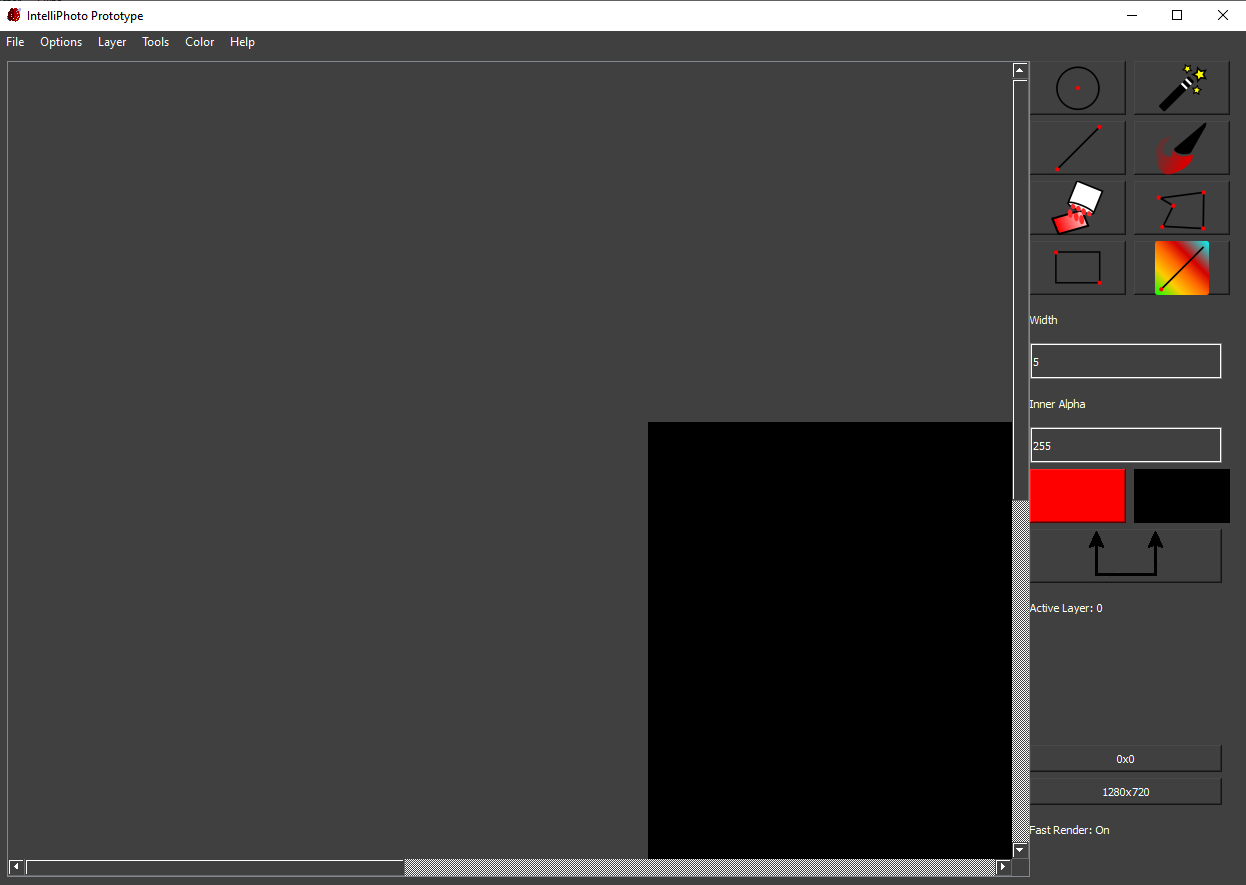
\includegraphics[width=0.55\linewidth,keepaspectratio]{assets/startup}
\end{center}

\subsection{Image setup}
\subsubsection{Loading images}
To load a preexisting image, click on \texttt{File} in the top menu bar and then on \texttt{Open...} in the appearing context menu.

A file explorer window opens. Navigate to the image you want to open and click on \texttt{Open}. The image will now be imported and displayed.

\subsubsection{Exporting images}
To save the current canvas as an image, click on \texttt{File} in the top menu bar then hover over \texttt{Save As} and click on your preferred file format in the appearing context menu.
\begin{center}
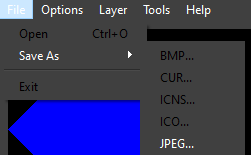
\includegraphics[width=0.3\linewidth,keepaspectratio]{assets/file-save}
\end{center}

A file explorer window opens. Navigate to your preferred save location, input a file name and click on \texttt{Save} or the equivalent in your system language. The image will be saved at that location in the selected file format.

\subsubsection{Saving projects}
To save the current project state click on \texttt{File > Save Project} or alternatively use the shortcut \texttt{CTRL+S} (or on \texttt{cmd+S} on MacOS). You may then select a location where to save your project.

\subsection{Working with layers}
\subsubsection{Creating a new layer}
To create a new layer, simply navigate to \texttt{Layer > Create Layer} and select the type of layer you want. Afterwards popups will appear, which will allow you to specify width and height of this new layer.
For Shaped Layers you afterwards have the option to specify the bounding polygon. To do this simply navigate to \texttt{Layer > Select Polygon Data} and create the polygon by clicking on the edge points on the canvas. The description of the usage under "Using the polygon tool" might help you.

\subsubsection{Setting the active layer}
The active layer is the layer you are currently editing. To change it, you currently have to specify the index of the layer under \texttt{Layer > Set Active}.

\subsubsection{Moving layers}
The layers are flexible and can be moved to a different position on the canvas, their order can be changed at will. For this you can use the movement options under \texttt{Layer}. Keep in mind that the changes always only effect the active layer you have chosen in the section "Setting the active layer". You can also alternatively use the shortcuts displayed unter this subsection.

\begin{center}
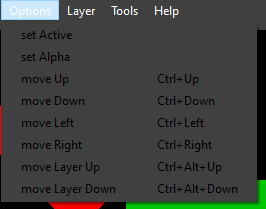
\includegraphics[width=0.3\linewidth,keepaspectratio]{assets/layer-options}
\end{center}

\subsubsection{Transparency and layers}
Layers can also be made more or less transparent under \texttt{Layer > set Alpha}. Values between 0 and 255 are valid. There is currently no error handling and this can lead to memory leaks, so be careful. This also only effects the active layer.

\subsection{Color Management}
\subsubsection{Setting the main and secondary color}
\begin{center}
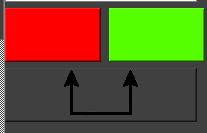
\includegraphics[width=0.3\linewidth,keepaspectratio]{assets/change-colors}
\end{center}
The main and secondary color are a concept used by all the drawing tools. You can set them individually, by clicking on the corresponding color icon on the right-hand-side toolbar, besides the canvas. The left color icon is for the main color, the right color icon for the secondary color.
After the click, a popup will appear. The popup will allow you to specify a new color.

\subsubsection{Switching main and secondary color}
An often desired use case is to switch the main and secondary color. So that you don't have to this manually, which would be time consuming there is an easy command to do it under the color icons on the right-hand-side toolbar, besides the canvas.
It is also bound to the keyboard shortcut \texttt{Ctrl+Alt+S}.

\subsubsection{Drawing with the pen tool}
To activate the pen tool simply click on the pen tool icon on the right-hand-side  toolbar.
To edit the active layer with the pen tool simply click and hold the left mouse button while hovering the layer on the canvas. When you click within the boundaries of the active layer, the pixels in the radius you selected will change their color to the main color which you selected under the section above.

\subsubsection{Drawing straight lines}
To activate the line tool just click on the line tool icon on the right-hand-side toolbar.
To draw a line you now have to left click on the starting point on the canvas, hold it pressed and move to the end point and release the mouse button. The width of the edge can be specified under \texttt{Width} in the right-hand-side toolbar.

\subsubsection{Drawing circles}
To activate the circle tool just click on the circle tool icon on the right-hand-side toolbar.
To create a circle you now have to left click and drag from the wanted center point, to some point on the edge of the circle you want, the circle will be previewed. You can release the mouse button after you are satisfied. Otherwise you can also click on the right mouse button while still holding the left one to cancel the operation.
The main color dictates the color of the edge, while the secondary color is used for the inside of the circle. If you want the inside to be transparent you can set the transparency on the side under \texttt{Inner Alpha} in the range between 0 (completely transparent) to 255 (completely opaque). The width of the edge can be specified under \texttt{Width}.

\subsubsection{Drawing rectangles}
To activate the rectangle tool click on the rectangle tool icon on the right-hand-side toolbar.
To create the a rectangle you now have to left click and drag form one wanted corner point to the other corner point diagonal from the starting point, the rectangle will be previewed. You can release the mouse button after you are satisfied.
Otherwise you can also click on the right mouse button while still holding the left one to cancel the operation.
The main color the color of the edge, while the secondary color is used for the inside of the recangle. If you want the inside to be transparent you can set the transparency on the side under \texttt{Inner Alpha} in the range between 0 (completely transparent) to 255 (completely opaque). The width of the edge can be specified under \texttt{Width}.

\subsubsection{Drawing polygons}
To activate the polygon tool click on the polygon tool icon on the right-hand-side toolbar.
To create the polygon you now have to left click on each of the corner points you want for your polygon in the order you want them to connect.
After you've all the points added, click close to the starting point you chose (You can see it in the preview.) to close up the polygon. You can end this process at any point by clicking the right mouse button.
The main color dictates the color of the edge, while the secondary color is used for the inside of the polygon. If you want the inside to be transparent you can set the transparency on the side under \texttt{Inner Alpha} in the range between 0 (completely transparent) to 255 (completely opaque). The width of the edge can be specified under \texttt{Width}.

\subsubsection{Using gradients}
To activate the gradient tool just click on the gradient tool icon on the right-hand-side toolbar. The gradient interpolates linearly from the main color to the second hand color. To change them refer to the section "Setting the main and secondary color".
The use of this tool is very similar to the line tool: Simply click and hold on the starting point of the gradient, move to the end location and release the mouse button. The pixels on the active layer will change accordingly.

\subsubsection{Fill the active layer in one color}
To activate the plain tool just click on the plain tool icon on the right-hand-side toolbar.
Afterwards you simply click inside of the canvas to fill the active layer with the main color.

\subsection{Closing the program}
To close the program you have to execute the exit program routine, which heavily depends on your operating system. Usually you can find a red cross symbol at the top right, though it may be different depending on your setup.
For Windows 10, the desired symbol looks like this when hovered:
\begin{center}

\includegraphics[width=0.9\linewidth,keepaspectratio]{assets/close-window}
\end{center}
Alternatively you can press \texttt{CTRL+Q} (Windows) (or \texttt{cmd+Q} on MacOS).

\end{document}
